% TEMPLATE for Usenix papers, specifically to meet requirements of
%  USENIX '05
% originally a template for producing IEEE-format articles using LaTeX.
%   written by Matthew Ward, CS Department, Worcester Polytechnic Institute.
% adapted by David Beazley for his excellent SWIG paper in Proceedings,
%   Tcl 96
% turned into a smartass generic template by De Clarke, with thanks to
%   both the above pioneers
% use at your own risk.  Complaints to /dev/null.
% make it two column with no page numbering, default is 10 point

% Munged by Fred Douglis <douglis@research.att.com> 10/97 to separate
% the .sty file from the LaTeX source template, so that people can
% more easily include the .sty file into an existing document.  Also
% changed to more closely follow the style guidelines as represented
% by the Word sample file. 

% Note that since 2010, USENIX does not require endnotes. If you want
% foot of page notes, don't include the endnotes package in the 
% usepackage command, below.

% This version uses the latex2e styles, not the very ancient 2.09 stuff.
\documentclass[letterpaper,twocolumn,10pt]{article}
\usepackage{usenix,epsfig}
\usepackage{amsfonts,amsthm,amsmath,amssymb}
\usepackage{array}
\usepackage{epsfig}
\usepackage{tikz}
\usepackage[hyphens]{url}
\usetikzlibrary{positioning}

\newtheorem{theorem}{Theorem}
\newtheorem{definition}[theorem]{Definition}
\begin{document}

%don't want date printed
\date{}
 
%make title bold and 14 pt font (Latex default is non-bold, 16 pt)
\title{\Large \bf Certificate Transparency With Better Privacy Guarantees}

%for single author (just remove % characters)
\author{
{\rm Your N.\ Here}\\
Institution
\and
{\rm Second Name}\\
Institution
\and
{\rm Third Name}\\
Institution
% copy the following lines to add more authors
% \and
% {\rm Name}\\
%Name Institution
} % end author

\maketitle

% Use the following at camera-ready time to suppress page numbers.
% Comment it out when you first submit the paper for review.
\thispagestyle{empty}


\subsection*{Abstract}
Your Abstract Text Goes Here.  Just a few facts.
Whet our appetites.

\section{Introduction}

Describe the problem CT solves, and how in one or two paragraphs.

\paragraph{Challenge: privately auditing the logs.} 
Explain that evidence of misbehaving log can compromise user privacy.

\paragraph{Challenge: non-public domains.}
Explain the problem with non-public domains in CT.

\paragraph{Our contribution.}
Briefly outline the two (three? short-lived certs) contributions, and explain the main idea.


\section{Preliminaries}

Before we describe our constructions, we first give some
background about certificate transparency, and the cryptographic primitives needed for our constructions. 

\subsection{Certificate Transparency}
Certificate Transparency (CT) \cite{CT,RFC} provides a way to catch CAs that distribute fraudulent certificates, either due to malicious intent or external compromise. It uses a public, untrusted, and append-only log to keep track of certificates that have been issued by various CAs so that CAs, domain owners, and users can keep track of what certificates have been issued and can catch inappropriate behavior on the part of CAs. In addition to policing the actions of CAs, CT provides means for catching and reporting logs that have failed to act in good faith and follow the rules of the protocol. Although it is possible to catch misbehavior in CT, the task of punishing CAs and logs must be carried out outside of the protocol, so proofs of misbehavior must be presented to an outside party with power to punish the transgressor.

The basic idea of CT is that when a CA wishes to issue a certificate, it sends the certificate to the log, who issues a signed timestamp of the certificate (Signed Certificate Timestamp, or SCT) which acts as a promise that the log will add the certificate within some short specified period of time called the maximum merge delay (MMD). The CA then distributes the certificate along with the SCT that attests it has been submitted to a log. Monitors and Auditors are two related forms of overseers that make sure changes to the log are being made appropriately and that any certificates distributed with SCTs are accurately registered in a log. Monitors are meant to have access to large amounts of resources in order to look at all of a log at once and seek out unauthorized certificates, while auditors are more concerned with checking the validity of individual certificates/SCTs and making sure a log is following the rules of the CT protocol.

The structure of the data structure in which log entries are stored is a Merkle tree where each leaf is a hash of a log entry. parties can make sure they have the same view of the tree by gossiping their most recent hash tree root, called a Signed Tree Head (STH). The proof of inclusion of an SCT in a log entry is the standard proof of inclusion for Merkle trees. The Merkle tree data structure always maintains a perfect tree, even when new entries are added. In order to prove that it has honored the append-only restriction, the log sends auditors/monitors a proof consisting of the nodes in the tree needed to construct the updated STH from the previous one. 

Our proposed solutions for privacy-preserving modifications to CT will leave the core of CT untouched but will require some additional information to be published in log entries and SCTs. Each solution will separately require different changes, but the alterations required by the two schemes are compatible with each other and can be implemented together. 

We will use the following notation and security definitions when proving the security of our zero-knowledge proof of log entry exclusion. Entries in a log are represented as tuples $(data, I, T)$ where $I$ and $T$ are integers representing an index and a timestamp respectively and $data$ abstractly represents the rest of the contents of the log entry (e.g. X509 certificate). We will refer to components of an entry with a subscript notation, so $T_x$ refers to the timestamp of a log entry $x$. An SCT is represented as a tuple $(data, T)$ with the index omitted, as an SCT, not yet being entered in the log at the time of issuance, does not have an index number.

\subsection{Cryptographic Primitives}
We will use a number of cryptographic primitives to achieve our privacy goals. Our secure redaction scheme will make use of a Verifiable Random Function (VRF) \cite{MRV99}, which is a function with public and private keys such that the holder of the private key can compute the function along with a proof that the function was computed correctly. Anyone with access to the public key and the proof can then verify that the function was in fact computed correctly. Our formation of the definition follows that of \cite{DY05}:
\begin{definition}[VRF]
A function family $F_{(\cdot)}$ is a family of VRFs (or just a VRF) if there exist efficient algorithms $(Gen, Eval, Verify)$ such that $Gen(\lambda)=(pk, sk)$, where $\lambda$ is a security parameter, $Eval_{sk}(x)=(F_{sk}(x), \pi_x)$ where $F_{sk}(x)$ is the function value and $\pi_x$ is the proof of correctness, and $Verify_{pk}(x,y,\pi)$ verifies that $y=F_{sk}(x)$ using the proof $\pi$. We require the following properties of $(Gen, Eval, Verify)$:
\begin{itemize}
\item \textbf{Uniqueness}: no values $(pk, x, y1, y2, \pi_1, \pi_2)$ can satisfy $Verify_{pk}(x, y_1, \pi_1) = Verify_{pk}(x, y_2, \pi_2)$.
\item \textbf{Provability}:  $Verify_{pk}(x,y,\pi)=1$ if and only if $(y,\pi)=Eval_{sk}(x)$.
\item \textbf{Pseudorandomness}: Any PPT adversary $A=(A_E,A_J)$ given oracle access to $(Gen, Eval, Verify)$ that does not query the VRF oracle on $x$ wins the following game with at most negligible advantage, where winning is defining as selecting $b'$ such that $b'=b$:
\begin{enumerate}
\item Run $Gen(\lambda)=(pk,sk)$.
\item Run $A_E^{Eval_{sk}(\cdot)}(pk)$ to obtain the tuple $(x, state)$.
\item Let $y_0=F_{sk}(x)$ and let $y_1\in_R\{0,1\}^n$ where $n$ is the output length of $F$.
\item Run $A_J^{Eval_{sk}(\cdot)}(y_b, state)$ to obtain $b'$.
\item Output $b'$.
\end{enumerate}
\end{itemize}
\end{definition}

One simple way to construct a VRF in the random oracle model makes use of a \textit{unique} signature scheme and a hash function, where the signed input is the proof and the hash of the signed input is the output. A unique signature scheme is defined as follows:
\begin{definition}[Unique Signature]
A signature scheme with unique signatures is a signature scheme $\sigma =$(G, Sign$_{sk}(msg)$, Verify$_{pk}(msg, sig)$) with the additional property that for each message $m$, there is exactly one $s$ such that Verify$_{pk}(m, s)=1$.
\end{definition}

Turning our attention to the tools needed for our proof of log exclusion, we note that although a random oracle will be more than enough to prove the soundness of our zero knowledge protocol, it should be pointed out that all that is really needed is a \emph{near collision resistant hash function}:
\begin{definition}[$\delta$-near collision resistant hash function]
A hash function $H: \{0,1\}^*\rightarrow \{0,1\}^n$ is $\delta$-near collision resistant if it is hard to find $x,y\in\{0,1\}^*$ such that $|H(x)-H(y)|<\delta$, where $H(x), H(y)$ are interpreted as integers.
\end{definition}
Although a stronger assumption than collision-resistance, it would appear that most hash functions conjectured to be collision-resistant also satisfy $poly(n)$-near collision resistance, where $poly(n)$ represents some polynomial function of $n$. It is also clear that any random function has $poly(n)$-collision resistance since the probability that two random points in $\{0,1\}^n$ fall within $poly(n)$ of each other is $\frac{poly(n)}{2^n}$.

\subsection{Security Model}
In order to develop our zero-knowledge proof of log exclusion, we will need to make some minor additions to the information kept by a CT log. These changes are described in more detail in section 3. Below we give a formalization of the definition of a CT log that has been modified to include our additional requirements. 
\begin{definition}[CT Log]
A CT log is an entity that maintains append-only lists Log, hashLog, ILog, and TLog as well as 4 signing keys $k_H, k_T, k_I, k_S$ and a counter $i$. A CT log's lists are initially empty, and the counter is initially set to 0. It also has access to $poly(\lambda)$-near collision resistant hash function $H$, a signature scheme $\sigma=(KeyGen, Sig, Vrfy)$ , and another signature scheme $\sigma_k = (KeyGen, Sig, Vrfy)$ with efficient proof of knowledge properties. Upon receiving a message $m, t$ from party $P$, a log takes the following actions\footnote{Although in reality it is the log who assigns $t$ and not $P$, defining the security model such that $P$ selects $t$ makes the adversary strictly more powerful in our setting.}:
\begin{itemize}
\item append $e = (m, i, t)$ to Log
\item append $(H(e), Sig_{k_H}(H(e)))$ to hashLog
\item append $(i+H(e), Sig_{k_I}(i+H(e)))$ to ILog
\item append $(t+H(e), Sig_{k_T}(t+H(e)))$ to TLog
\item send $P$ $(H(s), Sig_{k_H}(H(s)))$
\item send $P$ $(t+H(s), Sig_{k_T}(t+H(s)))$
\item send $P$ the SCT $s=(m, t)$ and $Sig_{k_S}(s)$
\item increment $i$ by one
\end{itemize}

A well-formed list Log consists of $poly(\lambda)$ entries ordered by increasing order of both $I$ and $T$. Values of $I$ must begin at zero and be incremented by one for each subsequent entry. Values of $T$ must fall within a range of $poly(\lambda)$ where $\lambda$ is a security parameter. Furthermore, the order of entries of $I$ and $T$ must correlate, that is, if $I_x>I_y$, then it must hold that $T_x>T_y$. Lists hashLog, ILog, and TLog have one entry per entry in Log and are sorted in the same way.

A CT log also responds to requests for entries in its lists with the requested information.
\end{definition}

One of the primary tasks we undertake is to construct a secure zero-knowledge exclusion proof. We will make use of the following proof of exclusion soundness game and security definition in proving the security of our proposed solution. 

\begin{definition}[$ProofExcl_{\Pi,A,V,L}(\lambda)$]
The proof of exclusion game is played by an adversary $A$ with a log $L$ and Verifier $V$ using protocol $\Pi$ and security parameter $\lambda$. $L$ maintains append-only lists \emph{Log} (a well-formed CT log), \emph{hashLog}, \emph{ILog}, \emph{TLog}, which are initially empty. $L$ also has a counter $i$ initialized to zero and signing keys. It consists of two phases:
\begin{enumerate}
\item $A$ interacts with $L$ in $poly(\lambda)$ rounds where in each round $A$ sends $L$ a message $(m, t)$ with the range of all $t$'s sent being at most $poly(\lambda)$ and each $t$ strictly greater than the previous one. After each round, $A$ retrieves from $L$ the new entry added to each lists $L$ holds.
\item $A$ interacts with $V$ according to $\Pi$ and then $V$ outputs a bit $b$.
\end{enumerate}
$A$ wins the game when $b=1$.
\end{definition}
\begin{definition}[Zero-Knowledge Exclusion Proof]
A zero-knowledge exclusion proof is an interactive protocol between a Prover $P$ with access to log entries $x,z$, SCT $y$, signatures $\sigma_{I_x+H(x)},$ $\sigma_{T_x+H(x)},$ $\sigma_{H(x)},$ $\sigma_{T_y+H(y)},$ $\sigma_{H(y)},$ $\sigma_{I_z+H(z)},$ $\sigma_{T_z+H(z)},$ and $\sigma_{H(z)}$ and a Verifier $V$ with access to the public keys corresponding to the signatures who outputs $1$ or $0$ at the end of their interaction. Both parties are given access to a log $L$ and a security parameter $\lambda$. We require the following properties from a secure exclusion proof:
\begin{enumerate}
\item \textbf{Completeness}: $\forall x,y,z$ $s.t.$ $I_x+1=I_z, T_x<T_y<T_z$, and $\sigma_m$ is a signature on $m$ for all signatures above, $V$ outputs 1.

\item \textbf{Soundness}: $\forall$ PPT Adversaries $A, Pr[ProofExcl_{\Pi,A,V,L}(\lambda)=1]\leq negl(\lambda)$.

\item \textbf{Zero-Knowledge}: There exists an efficient simulator $S$ that, given only $\lambda$, can generate a transcript indistinguishable from that of the interaction between $P$ and $V$.
\end{enumerate}
\end{definition}
We will use the standard definitions of digital signature schemes and cryptographic commitments except where noted otherwise.


\section{Zero Knowledge Proof of Exclusion}
In this section, we present an efficient zero-knowledge proof that an SCT has not been entered into a Certificate Transparency (CT) log. Our proof allows an auditor (representing a web browser or user) to prove to an outside authority with power to investigate/punish the log that it holds an SCT $y$ whose timestamp falls between two neighboring log entries $x$ and $z$ and is therefore missing from the log, all without revealing $x$, $y$, or $z$. We begin by discussing the nature of the problem and the degree of privacy to be expected from a solution before presenting our construction in detail. 

\subsection{Discussion of Privacy Goals}
Recall that the auditor in our proof wishes to prove to a verifier that it holds an SCT $y$ whose timestamp falls between two neighboring log entries $x$ and $z$ without revealing $x$, $y$, or $z$. While it is clear why revealing the missing SCT $y$ would reveal information about the auditor's web browsing, it may not be immediately obvious why $x$ and $z$ should also be hidden: knowledge of the timestamps of $x$ and $z$ would allow a verifier interested in finding users who have visited some particular site (e.g. \emph{antigovconspiracy.net}) to visit that site and check if its SCT timestamp does indeed fall between those of $x$ and $z$, thus indirectly revealing information about the likely identity of $y$. We emphasize that it is important not only to prevent leaking information about the prover's private browsing during the protocol but also to avoid giving the verifier information it could use on its own to uncover the sites visited by the prover.

This raises the concern that in a case where a log has omitted only one SCT or a small set of SCTs, an exhaustive search of public SCTs may reveal which SCT has been excluded and compromise the privacy of the auditor. Since SCTs are publicly available to visitors of sites, this issue is intrinsic to CT if we want to be able to catch a log that has excluded a single SCT. Despite this necessary shortcoming, our approach provides the best possible privacy achievable in proving a CT log has misbehaved.

One could imagine an alternative solution that compromises by allowing a few missing SCTs to be ignored before allowing the proof to be completed and implicating a log, but even such a compromise scheme is unfortunately too much to ask. This can be illustrated through an example. If a scheme were to exist that would require, say, 100 SCTs to be missing before a log was implicated, thereby concealing the site visited by each prover among many others, a malicious log could game the system to break the user's privacy. It could omit the SCT of a site the user visited as well as 99 other SCTs for certificates it had issued itself. Then after the user proves the absence of 1 SCT, the log supplies proofs for the other 99 SCTs. This would complete the proof that the log had omitted an SCT, but it would also break the expected privacy of the user, making it obvious which site she had visited. In light of this necessary limitation to any proof of a cheating log, a particularly paranoid prover could additionally use a means of anonymization such as tor to hide her identity from the verifier. 

Since a zero knowledge proof by design hides all information about the log's infraction except that some SCT was missing, we note that this creates a problem for investigators and for a log that has been compromised. Once a log has been shown to have excluded SCTs, it must launch some internal investigation to determine the source of the problem and satisfy investigators that it will continue to operate in good faith. At the very least, if no information regarding the missing log entries can be found, a log can conclude that it has been compromised and make sure to change it's keys for future operation. 

A final note before presenting the construction: it may be objected that since there is an amount of time, the MMD, after an SCT is issued and before it is required to be in the log, there may be ``false positives'' where it is possible for a certificate with a valid SCT to not be included in the log. Our solution does not fall victim to this problem because, as will be seen, we require there to be entries already in the log both before and after the missing entry in order to complete the proof. 

\subsection{Construction}
Our construction requires the following additional components in the CT protocol:
\begin{itemize}
\item Each log entry $x$ is accompanied by signed messages $sig_{k_H}(H(x))$, $sig_{k_T}(T_x+H(x))$, and $sig_{k_I}(I_x+H(x))$ where $T_x$ is the SCT timestamp for $x$, $I_x$ is the index number of $x$ in the log, and $k_H, k_T,$ and $k_I$ are different signing keys. Including the index number should not be difficult since logs are already queried by index to receive entries. Each SCT $y$ is accompanied only by signed messages $H(y)$ and $T_y+H(y)$ since it may be impractical to give an SCT an index number before it is incorporated into the log. In total, this requires 5 additional signed messages to be distributed by the log for each certificate.

\item Monitors must make sure that the ordering of index numbers corresponds to the order of timestamps in log entries. That is, logs must ensure that if $I_x>I_y$, then it must hold that $T_x>T_y$. This ensures that the logs fulfill our definition of being well-formed and contrasts with the current setting where indexes can be assigned to queued entries in any order in a sequencing phase after SCTs are distributed. 
\end{itemize}

Protocol $\Pi$ is between an auditor/web user who has an SCT missing from the log and an outside verifier with capabilities to somehow punish the log. We require a commitment scheme that is additively homomorphic and allows for zero knowledge range queries and equality tests. These are achieved by various commitments and protocols such as the commitments of \cite{Ped92} or \cite{DF01} and the protocols in \cite{CM01}, \cite{Bou00}, \cite{DBB+15}, \cite{CP93}, \cite{Sch91}, \cite{Bra97}, \cite{CEvdG87}, and \cite{CCS08}. Additionally, we need a signature scheme for which it is possible to efficiently prove in zero knowledge that $c_1$ is a commitment to a signature on the content of commitment $c_2$. All of these properties are provided by the signature schemes presented in \cite{CL02} and \cite{CL04}, the latter of which claims that \cite{BBS04} can also be modified to suit our purposes. $H: \{0,1\}^*\rightarrow\{0,1\}^\lambda$ is a $poly(\lambda)$-near collision resistant hash function, and $\lambda$ is a security parameter.

The zero knowledge proof is in two parts. In the first part (summarized in figure \ref{picture}), the verifier receives commitments $C_{T_x}$, $C_{I_x}$, $C_{T_y}$, $C_{T_z}$, and $C_{I_z}$ to the indexes $I$ and timestamps $T$ of log entries $x, z$ and SCT $y$. The second part proves that the indexes are adjacent and that the timestamps are ordered such that $T_x<T_y<T_z$.

The idea for the first part is to use the signed messages accompanying a log entry to both verify that the commitments given by the prover are legitimate and to prove that the each index, timestamp pair actually corresponds to the same log entry. While under a commitment, both $I_x$ and $T_x$ are added to $H(x)$, giving commitments to $I_x+H(x)$ and $T_x+H(x)$. We can then prove in zero knowledge that these commitments and the commitment to $H(x)$ correspond to commitments to the signed messages from the log. 

To complete the actual proof of omission, the prover sends and reveals a commitment $C_1$ to the number $1$ and proves in zero knowledge that $C_{I_x+1}$ and $C_{I_z}$ are commitments to the same value. Next the verifier computes commitments $C_{p_1}=C_{T_z-T_y}$ and $C_{p_2}=C_{T_y-T_x}$. Finally the prover proves in zero knowledge that $p_1>0$ and $p_2>0$. The complete protocol is as follows:

\begin{enumerate}
\item Prover sends commitments $C_{sig_{k_I}(I_x+H(x))}$, $C_{sig_{k_H}(H(x))}$, $C_{sig_{k_T}(T_x+H(x))}$,  $C_{sig_{k_H}(H(y))}$, $C_{sig_{k_T}(T_y+H(y))}$, $C_{sig_{k_I}(I_z+H(z))}$, $C_{sig_{k_H}(H(z))}$, $C_{sig_{k_T}(T_z+H(z))}$, $C_{T_x}$, $C_{H(x)}$, $C_{I_x}$, $C_{H(y)}$, $C_{T_y}$, $C_{T_z}$, $C_{H(z)}$, $C_{I_z}$, $C_1$, and $r_{C_1}$.

\item Verifier computes $C_{I_x+H(x)}$, $C_{T_x+H(x)}$, $C_{T_y+H(y)}$, $C_{I_z+H(z)}$, and $C_{T_z+H(z)}$

\item Prover proves in zero knowledge that each commitment to a signature in step 1 corresponds to the correct value (as shown in figure \ref{picture}).

\item Verifier computes $C_{I_x+1}$, $C_{p_1}=C_{T_z-T_y}$, and $C_{p_2}=C_{T_y-T_x}$.

\item Proves proves in zero knowledge that $I_x+1=I_z$, $p_1>0$, and $p_2>0$.
\end{enumerate}

\begin{figure}
\centering
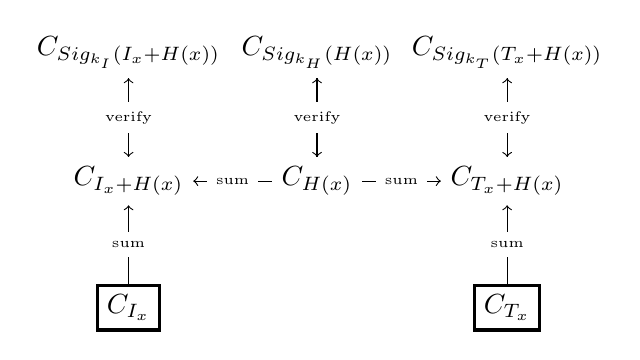
\begin{tikzpicture}
\node (sighash) {$C_{Sig_{k_H}(H(x))}$};
\node (hash) [below=of sighash] {$C_{H(x)}$} ;
\node (Thash) [right=of hash]{$C_{T_x+H(x)}$};
\node [style=rectangle, draw=black, very thick] (T) [below=of Thash] {$C_{T_x}$};
\node (sigT) [above =of Thash] {$C_{Sig_{k_T}(T_x+H(x))}$};

\node (Ihash) [left=of hash]{$C_{I_x+H(x)}$};
\node [style=rectangle, draw=black, very thick] (I) [below=of Ihash] {$C_{I_x}$};
\node (sigI) [above =of Ihash] {$C_{Sig_{k_I}(I_x+H(x))}$};

\draw[->] (hash.east) to node[fill=white] {\tiny sum} (Thash.west);
\draw[->] (hash.north) to node[fill=white] {\tiny verify} (sighash.south);
\draw[->] (Thash.north) to node[fill=white] {\tiny verify} (sigT.south);
\draw[->] (T.north) to node[fill=white] {\tiny sum} (Thash.south);
\draw[->] (sigT.south) to node[fill=white] {\tiny verify} (Thash.north);


\draw[->] (hash.west) to node[fill=white] {\tiny sum} (Ihash.east);
\draw[->] (sighash.south) to node[fill=white] {\tiny verify} (hash.north);
\draw[->] (sigI.south) to node[fill=white] {\tiny verify} (Ihash.north);
\draw[->] (I.north) to node[fill=white] {\tiny sum} (Ihash.south);
\draw[->] (Ihash.north) to node[fill=white] {\tiny verify} (sigI.south);

\end{tikzpicture}

\caption{The process of getting verified commitments to the Index and Timestamp of a log entry. The diagram for an SCT would be the same except without the left-hand column.}
\label{picture}
\end{figure}
\subsection{Proof}
\begin{theorem}
If $H$ is a $poly(\lambda)$-near collision resistant hash function and the signature scheme used is existentially unforgeable and allows for efficient proofs of knowledge of a signature, then $\Pi$ is a secure Zero-Knowledge Exclusion Proof. 
\end{theorem}
\begin{proof}
\textbf{Completeness}. The completeness of the proof follows directly from the construction. Any auditor with access to an SCT $y$ with the given properties that has access to the log can follow the protocol and convince a verifier that the log is cheating.\\

\textbf{Soundness}. We prove that no adversary $A$ can win the security game $ProofExcl$ with greater than negligible probability through a series of three hybrids:
\begin{itemize}
\item \emph{hybrid 0:} The security game $ProofExcl_{\Pi,A,V,L}(\lambda)$.
\item \emph{hybrid 1:} Same as hybrid 0, except after $V$ outputs $b$, we run the extractor for each proof of knowledge of a signature and output 0 if any of the extractions fail. This is indistinguishable from hybrid 0 by the extractability property of the proof of knowledge of a signature. Since the proof of knowledge protocol has an efficient extractor, we will never fail to extract the signatures used.
\item \emph{hybrid 2:} Same as hybrid 1, except after the verification of the extractions, we check the extracted signatures and output 0 if any of them are not found in the corresponding list held by $L$: either Log, hashLog, ILog, or TLog. This hybrid follows from hybrid 1 due to the existential unforgeability of the signature scheme. If $A$ could ever output zero based on this additional check, we could construct a new adversary $B$ that breaks the existential unforgeability of the signature scheme by running $A$ until it outputs 0 on this check and then outputting the signature $s$ that was not found in the log. Since all signatures made by $L$ are in one of the lists, $s$ must be a forged signature. Thus the additional check in this hybrid will never cause an output of 0 when $b=1$. 
\end{itemize}
Now we prove that no adversary $A$ can win hybrid game 2 with more than negligible probability. Note that we only need to prove the soundness for the first part of the protocol, as soundness for the second part of the protocol follows from the soundness of the various zero knowledge proofs it uses as subroutines. That is, we need only to show that no adversary $A$ can fake the indexes or timestamps of signed entries from $L$. We show here the proof for indexes; the proof for timestamps is almost identical. 

In order for an adversary $A$ to fraudulently win the game, it must produce commitments $C_{I_x''+H(x')}$, $C_{I_x^*+H(x^*)}$, $C_{I_z''+H(z')}$, and $C_{I_z^*+H(z^*)}$ such that the following conditions hold:
\begin{itemize}
\item $I_{x''}+1=I_{z''}$
\item $I_{x^*}+H(x^*)=I_{x''}+H(x')$
\item $I_{z^*}+H(z^*)=I_{z''}+H(z')$
\item $(I_{x''}+H(x'), Sig_{k_I}(I_{x''}+H(x'))\in$ ILog
\item $(I_{z''}+H(z'), Sig_{k_I}(I_{z''}+H(z'))\in$ ILog
\item $x'\neq x''$ OR $z'\neq z''$
\end{itemize}
We will consider the case where $x'\neq x''$. The case for $z'\neq z''$ is identical. If the adversary succeeds, then it must have found values $I_{x^*}, x^*, I_{x''}, x'$ such that 
\begin{align}I_{x^*}+H(x^*)=I_{x''}+H(x')\end{align}
Define $d=I_{x''}-I_{x*}$. Then we have that 
\begin{align}H(x^*)=H(x')+d \end{align} 
But $d < poly(\lambda)$ since $A$ can only send polynomially many messages to $L$ to populate the log. Thus we can define adversary $B$ that breaks the $d$-near collision resistance of $H$ by calling $A$ as a subroutine, using the extractors from the zero knowledge proofs in the second part of the protocol to retrieve the contents of the commitments $A$ used, and outputting $x^*, x'$ as its near collision. 

\textbf{Zero-Knowledge}. The zero knowledge property is easy to establish as the sequential composition of a series of other zero knowledge proofs. The simulator starts by committing to a series of random values (except the commitment/reveal to 1, which is done honestly). After the verifier computes the appropriate sums of commitments, the simulator sequentially executes several copies of the simulator of ``knowledge of a signature'' from \cite{CL04} or \cite{CL02} depending on the signature scheme used. After the remaining computations on the commitments by the verifier, the simulator finally runs the simulator for the proof of equality of committed values and the two range proofs.
\end{proof}

\subsection{Alternative Construction}

A similar zero knowledge proof $\Pi'$ exists that relies only on the collision resistance of $H$. It is similar to $\Pi$, except instead of having signatures on $I_x+H(x)$ and $T_x+H(x)$, the log publishes signatures on $I_x||H(x)$ and $T_x||H(x)$. Before adding $T_x$ or $I_x$ to $H(x)$, the verifier multiplies each by a commitment to $2^n$, effectively left-shifting $T_x$ and $I_x$ so the sum with $H(x)$ can be interpreted as a concatenation of the two values. This simplifies the soundness proof so that the value of $d$ will always be 0, and any adversary $A'$ winning the modified security game could be used by another adversary $B'$ to find a collision for $H$. The proof that $\Pi'$ is a zero-knowledge proof is otherwise very similar to that of $\Pi$ and can be omitted. Although the soundness of $\Pi'$ relies on a weaker assumption than $\Pi$, it requires the prover to send an additional commitment to the verifier and for the prover and verifier to compute two interactive multiplications on commitments \cite{CM01}, rendering $\Pi'$ the less practical variant of the proof.

\subsection{Privacy Compromise with Actionable Proof of Exclusion}

Although we have presented a solution that is optimal in terms of privacy, it is possible that there exist other desirable solutions that compromise on privacy in order to provide other useful functionalities that render them more suitable for deployment. In particular, we are interested in the case where the verifier would like to have some recourse other than completely distrusting a log after learning that it has cheated. The best a verifier could do using our scheme as stated is to distribute a whitelist consisting of certificates that it has seen on the log and instruct browsers to reject any SCT from that log for other certificates. It is possible, however, to do somewhat better if we are willing to compromise on the degree of privacy we hope to achieve.

Since it is likely that any SCT excluded from the log but publicly available on the internet will be caught by a verifier (e.g. Google) without need for a proof, we note that we must mainly concern ourselves with SCTs for certificates that will not be publicly available. In this light, we hope for a scheme where the verifier does not learn the domain of the bad SCT but is given the ability to provide other users with the ability to check if they encounter it. We achieve this by relaxing our privacy goals to a variant of witness-indistinguishability in which the proof provided will be witness indistinguishable except with the modification that a verifier holding the witness used to construct the proof can learn that the proof was computed with that particular witness. This notion is clearly only useful if witnesses are computationally hard to find.

We need only to make a slight modification to our zero knowledge protocol in order to achieve this weakened notion of witness indistinguishability. We set the randomness $r$ used in the pedersen commitment to the  hash $x$ of the missing SCT to zero. This gives us a weakened commitment of the form $c=g^x$, which is still hiding because of the high entropy of $x$, the hash output. The rest of the proof proceeds as before. Now the verifier can distribute $c,g$, and any browser can check if an SCT it has acquired matches the one used to construct the proof. 

\subsection{Practical Considerations}

The presented solution can be implemented on top of the existing Certificate Transparency specification, RFC6962, with some adjustments.

\textbf{Key Distribution}: The existing mechanisms for distributing the log's key for signing SCTs can be used for distributing the three additional keys. TODO(eranm): Refer to the keys in the same way as above.

\textbf{Obtaining Entries around timestamp}: The current CT RFC only specifies an API for getting the index of an entry in the log given its hash, requiring the client to know the timestamp and the certificate for that entry. A new API endpoint can be added to return a number of log entries around a timestamp specified by the client.
TODO(eranm): More accurate specification of the inputs and outputs of the needed API, including the keys.

\textbf{Adding signatures to SCTs}: Signed Certificate Timestamps have an extensions field which can be used for embedding the signatures $\sigma_{T_y+H(y)},$ $\sigma_{H(y)}, $. As the signature in the Signed Certificate Timestamp covers the extensions field, these signatures should be produced before the signature over the entire Signed Certificate Timestamp TODO(eranm): Notation for the signature over the entire SCT.

Timestamps are required to be unique under this construction. Distributed implementation of a log could issue two SCTs with exactly the same timestamp for two different entries submitted at the same time. To avoid the restricting the implementation, each front-end of the log will be assigned a unique ID, which will be concatenated to the timestamp to ensure uniqueness. In practice, the unique ID should be added as an extension to the SCT to avoid changing the timestamp format currently specified in the CT RFC.

\subsection{Performance Estimates}
\begin{center}
\begin{figure*}
    \begin{tabular}{ | l | l | l | l |}
    \hline
    Component & Proof Size (bytes) & Prover Time (ms) & Verifier Time (ms) \\ \hline
    Signature Verification (8x) & 45270 & 712.4 & 324.9 \\ \hline
    Rest of Proof & 16328 & 30.6 & 36.2 \\ \hline
    Total & 378486 & 5729.8 & 2635.1 \\
    \hline
    \end{tabular}
    \caption{Running times and proof size for ZKPDL implementation of our protocol using the signatures of \cite{CL02}. The values for verifying the 8 signatures are separated from the rest of the protocol to reveal the source of costs.}
\label{ZKP_perf}
\end{figure*}
\end{center}

\begin{center}
\begin{figure*}
    \begin{tabular}{ | l | l | l |}
    \hline
    Signature & Log Entry Growth (bytes) & SCT Growth (bytes) \\ \hline
    CL02\cite{CL02} & 1791 & 1194 \\ \hline
    BBS\cite{BBS04} & 480 & 320 \\ 
    \hline
    \end{tabular}
    \caption{Expected growth in log entry and SCT size due to inclusion of signatures required for our scheme when using CL02 signatures or BBS signatures. Log entries require including 3 signatures, and SCTs require 2.}
\label{ZKP_bloat}
\end{figure*}
\end{center}
We implemented a prototype of our protocol in parts using ZKPDL \cite{ZKPDL} for the purpose of estimating the performance of such a scheme and ran it on a consumer laptop equipped with an intel i5 Sandy Bridge processor. Our implementation consisted of the entire protocol except the verification of the signatures, for which a ZKPDL implementation already exists for the RSA-based signature scheme of \cite{CL02}. Using 2048-bit RSA keys, we measured the proof size, prover computation time, and verifier computation time for our implementation as well as the signature verification (which we multiply by 8 to account for the 8 verifications needed in the proof). The numbers shown in figure \ref{ZKP_perf} are averages over 20 executions. Although the protocol may seem costly, we point out that it is meant to be one which is executed infrequently to catch cheating logs and is not expected to be used as part of regular day to day web browsing activities. As such, the cost of under 10 seconds and 400kb on the network seems reasonable. It is important to note that the 400kb proof is not something that will be included in SCTs or logs but data that is generated when the proof is needed. The overhead in terms of growth of SCTs and log entries is shown in figure \ref{ZKP_bloat}. These numbers, especially those for BBS signatures, are very reasonable when it is considered that the SCTs will typically be delivered along with certificate chains that are already sometimes several kilobytes large. 

\section{Private domains in CT}

A drawback of CT as currently formulated is that every SCT and log entry reveals the name of the domain for which the associated certificate is issued. This creates a problem for companies who wish to have certificates issued for internal domains without revealing the existence of the internal domains to monitors and auditors of the log. A great deal of discussion has taken place around this issue (\cite{redaction-disc}), the main proposed solutions to which are redaction of names via wildcards (\cite{RFC-bis}) or including a hash of domain names instead of the names themselves. The former solution does not fix the subdomain specified by a wildcard, meaning that it does not offer optimal precision or privacy, and the latter is vulnerable to a dictionary attack where an adversary could guess possible domain names until a correct one is found. This attack should be easy to carry out because domain names are typically very low-entropy and can be guessed. We set out to modify the CT scheme so as to allow for companies with internal domains to take advantage of its benefits without revealing any private information. We believe our solution strikes an ideal balance between transparency and privacy without requiring any major or impractical changes to the functioning of a CT log.

Our solution uses Verifiable Random Functions to allow privileged internal users access to CT log information regarding company-issued certificates without revealing anything to the public. The main insight of this section is that VRFs are a perfect fit for the needs of a secure redaction scheme in CT. In the variation of CT described below, instead of the name of the domain, a token derived from the name is publicly listed\footnote{It is also possible to replace only part of the domain name instead of the whole name if desired.}. The domain owner has a proof it can give to site visitors that allows anyone with a copy to both find log entries associated with the domain and to verify that certificates issued for that domain are indeed linked to a given SCT. Our construction requires only a Verifiable Random Function \cite{MRV99} which can be constructed in the random oracle model from a collision-resistant hash function and a unique signature scheme, as observed by \cite{MBB+15}. RSA \cite{RSA78} and BLS \cite{BLS01} signatures are both unique, so either can be used to implement our changes. \cite{MBB+15} also presents a different, discrete-log based VRF that is equally applicable here and whose security follows from the DDH assumption. The VRF they use has $F_k(x)=H(x)^k$ and proves that the value was computed correctly with a Chaum-Pedersen proof of equality for two discrete logarithms.

\subsection{Construction}
The construction is simple. The domain owner $D$ will use a VRF $\nu$ to generate secret and public keys $sk_\nu$, $pk_\nu$ respectively. Each CA additionally has its own signing key pair $sk_C, pk_C$. When $D$ requests a certificate for domain $d$ from a CA, $D$ selects a salt\footnote{The salt could be omitted from the scheme but is useful in the case that the key $sk_\nu$ is stolen. In this case, the holder of $sk_nu$ can mount a dictionary attack against each token $t$ on the log. Including a salt means that a separate attack must be made for each entry instead of making one for all entries from $D$.} $s$ computes $(t, \pi)=Eval_{sk_\nu}(d||s)$ and sends to the CA the token $t$, $s$, $pk_\nu$, and $d$. The CA then sends the log $t$, a signature $\sigma=(pk_\nu, Sign_{sk_C}(pk_\nu))$, $s$, and $D$. The log creates an SCT that includes $t$, $\sigma$, $s$, $D$ and returns it to the CA who gives the SCT to the domain owner along with the certificate. The log includes, $t$, $\sigma$, $s$, and $D$ in the corresponding log entry. $D$ distributes $d$, $\pi$ to any site visitor, auditor or monitor it desires. This could mean either posting $\pi$ publicly or only distributing it among employees who need access.

The principal benefit of this modification is that an observer without access to $\pi$ is unable to detect the existence of domain $d$. As this modification otherwise leaves CT largely unchanged, it remains only to show how an auditor can check that a given SCT is valid and how a monitor can be convinced that there are no fraudulent certificates issued for $d$:
\begin{itemize}
\item\textbf{Monitor}: A monitor with access to $\pi$ can check that $Verify_{pk_\nu}(d,t,\pi)=1$ and then find all log entries that include $t$, verifying that they are all legitimate just as it could do before. Monitors must additionally check that there is only ever one $\sigma$ associated with each domain owner in order to catch anyone masquerading as that domain owner using a different key pair.
\item\textbf{Auditor}: As in the case for the monitor, an auditor can check $Verify_{pk_\nu}(d,t,\pi)=1$ to verify that the token $t$ included with a certificate is indeed associated with the domain name that is the subject of the certificate. 
\end{itemize}

\subsection{A Second Solution}
There exists a second solution that follows a similar approach, but completely hides the name of the domain owner to whom a certificate is being issued. It is even simpler than the first solution, but the cost of the additional privacy is that the log sees the name of the domain which is the subject of the certificate and therefore needs to be trusted not to leak it. In this variant, any SCT, log entry, or certificate issued for domain $d$ will include the token $t$ computed by the log. When a certificate is created, the domain owner is given the proof $\pi$ by the log. The domain owner still distributes $\pi$ to any privileged auditor or monitor.

As before, an outside user without access to $\pi$ is unable to detect the existence of domain $d$. Additionally, it is not even visible that a certificate has been issued to the domain holder. The tasks for monitors and auditors are the same as before, except that monitors need not verify the connection between $s$ and the domain owner since neither appear in the log. Note that since the signature scheme used is unique, it is not possible for a malicious log to use more than one signature for the same domain name and hide illicit certificates from the eyes of the monitor. 

\subsection{Performance Estimates}
\begin{center}
\begin{figure*}
    \begin{tabular}{ | l | l | l | l | l |}
    \hline
    Signature & Proof Size (bytes) & Output Size (bytes) & Computation Time (ms) & Verification Time (ms) \\ \hline
    BLS & 64 & 32 & 12.10 & 12.89 \\ \hline
    RSA & 256 & 32 & 4.91 & 0.16 \\
    \hline
    \end{tabular}
    \caption{Comparison of VRF implementations using BLS and RSA signatures with SHA256 hashes. The BLS signatures were built using the PBC library, and the RSA signatures are from OpenSSL.}
\label{VRF_perf}
\end{figure*}
\end{center}
\begin{center}
\begin{figure*}
    \begin{tabular}{ | l | l | l |}
    \hline
    Signature & Log Entry Growth (bytes) & SCT Growth (bytes) \\ \hline
    BLS & 206 & 272 \\ \hline
    RSA & 400 & 656 \\
    \hline
    \end{tabular}
    \caption{Additional data needed to be stored in SCTs and log entries, in bytes. Not included are the names of the top-level domain and overhead due to additional fields. Log entries do not include the VRF proof, but the additional data needed to be stored in entries and SCTs are otherwise the same.}
\label{VRF_bloat}
\end{figure*}
\end{center}
We implemented VRFs using both BLS and RSA signatures. We built the BLS signatures from the PBC library \cite{PBC} using the default type A parameters and used the (2048-bit) RSA and SHA256 functions made available by OpenSSL. We ran our VRF code on a consumer laptop equipped with an intel i5 Sandy Bridge processor, and our performance results over 20 evaluations and verifications of the VRF on input ``mySecret.domain.com''\footnote{The first step of the BLS signature is to hash the input, so the choice of domain name is unimportant.} are shown in figure \ref{VRF_perf}. The proof size listed is the size of the respective signature, and the output size is the same because both outputs are simply the evaluation of SHA256 on the signatures. Although the VRF based on RSA is faster, the BLS-based VRF saves a great deal of space without taking unreasonably long to compute. The difference in size between the two signatures also entirely explains the differences in growth to log entry and SCT sizes shown in figure \ref{VRF_bloat}. The small size of the BLS-based VRF recommends it as an excellent choice for adoption in practice. As mentioned above, the additional data stored in log entries will include the name of the domain owner, the output of the VRF, the VRF public key used by the domain owner, a 32-bit salt, and a signature on the VRF public key (we assumed ECDSA signatures in estimating size). SCTs will additionally include the VRF proof.

\section{Short-Lived Certificates in CT}
We considered the interaction of Certificate Transparency with another proposed improvement to the web's public-key infrastructure: short-lived certificates \cite{Riv98}. The fundamental idea behind short-lived certificates is to issue certificates with relatively short validity periods in order to remove the need on the part of a client to check whether or not a certificate received continues to be valid. Instead of revoking a certificate, the domain owner in the short-lived certificate setting simply refrains from issuing a new short-lived certificate in the event of key compromise. \cite{TSH+12} explores the details of this idea and compares it favorably to other proposed and implemented solutions for certificate revocation. 

Considering the possibility of applying short-lived certificates in conjunction with certificate transparency presents the new difficulty of avoiding bloated log sizes. The frequency with which new certificates would need to be issued under the short-lived certificate regime would mean that where one log entry would suffice for a regular certificate, nearly 100 short-lived certificates would be needed. A naive integration of the two solutions would lead to log sizes far larger than is truly necessary, but a simple solution can remedy this issue and allow the two solutions to work together quite well. Instead of creating one log entry per certificate for short-lived certificates, a large number of potential short-lived certificates will be allotted one log entry. This log entry will have a special flag set to indicate that it corresponds to a family of short-lived certificates, and the validity period for the log entry will be comparable to that of a regular, long-lived certificate. An auditor in possession of a short-lived certificate would know to accept any short-lived certificate whose validity range falls within the range of the corresponding long-lived SCT/log entry. This gives rise to a best-of-both-worlds scenario where the growth of the CT log is no different from that of a regular certificate, but the short-lived nature of the individual certificates also resolve revocation issues.

\section{Related Work}

Well-documented concerns about the state of the web's public-key infrastructure (PKI) \cite{CO13} have led to a number of proposed solutions for improving the capacity for catching problematic CAs or dispensing with CAs altogether. Pinning solutions such as Tack \cite{Tack} improve security by adding a ``pinned'' signing key that is associated with a server and without which the server will not be considered authentic. In addition to CT, there are a handful of other proposed PKI improvements that rely on the concepts of transparency of logs. The EFF's Sovereign Keys proposal uses a log to list the Sovereign Keys associated with domains and allows for automatically routing around certain certficate-related attacks where users tend to click through browser warnings. \cite{SovKeys}. AKI and ARPKI implement a set of checks and balances to prevent problems rooted in the misbehavior of one or a few CAs, and ARPKI is co-designed with a formal model to prove its security properties \cite{KHP+13}\cite{BCK+14}. Namecoin uses a blockchain to achieve similar goals as other improved PKI schemes \cite{Namecoin}.

Certificate Transparency has received heightened academic attention as it begins to be widely deployed in Chrome and Chromium browsers. Multiple works have analyzed the security of Certificate Transparency and its generalizations or designed efficient protocols for parts of the design that are not specified in the current RFC. \cite{CSP+15} provides efficient gossip protocols to ensure that different users of CT do in fact have the same view of the logs with which they interact. \cite{DGHS16} formally proves the security of many aspects of Certificate transparency, and \cite{CM16} proves the security of a generalization of Certificate Transparency they call ``Transparency Overlays,'' which can be added on top of other protocols such as Bitcoin to add a layer of transparency.  \cite{CM16} leaves the exploration of the interaction between transparency and privacy as an interesting open problem, one which our work begins to study. 

The notion of transparency itself has been studied in various settings not necessarily related to the web's PKI and appears to be a fairly general notion. Revocation Transparency provides a transparency-based solution for certificate revocation \cite{RevTrans}. DECIM \cite{YRK15} uses a transparency log to keep track of uses of a public key in a messaging context, thereby enabling its owner to detect key misuse. \cite{FDP+14} improves the security of mobile app distribution with ``Application Transparency.''  Extended Certificate Transparency \cite{Rya14} adds to CT the ability handle certificate revocation and presents an application to secure email. Coniks \cite{MBB+15} uses Key Transparency to build a secure messaging scheme. Finally, a number of works have focused on building general transparent data structures and enabling computation over them \cite{Insynd}\cite{Balloon}\cite{Versum}. 

\section{Conclusion}
We have examined various elements of Certificate Transparency with the goal of applying cryptographic solutions to remedy the compromise of private information without significantly disrupting the operation of CT as it is currently designed. Our primary goals were to securely redact private domain names in CT logs and to develop a privacy-preserving means of exposing logs that have excluded certificates after issuing certificates for them. We accomplished the former goal by observing that the security properties of a VRF, when applied appropriately to the setting of CT, provide exactly the privacy properties desired of a domain name redaction scheme. The latter problem was resolved by developing a zero knowledge proof that achieves the best possible security for privately implicating a cheating log. It is our hope that these practical solutions based on widely-used cryptographic primitives can be used to promote a more transparent web without any compromise in user privacy. 

\section{Acknowledgments}

A polite author always includes acknowledgments.  Thank everyone,
especially those who funded the work. 

\section{Availability}

Our VRF implementation is available at \url{https://github.com/SabaEskandarian/simpleVRF}, and the simulation code for the second part of our zero knowledge proof of exclusion can be found at \url{https://gist.github.com/SabaEskandarian/2217f2ce8b8a8ca6c6f8732a584c49e8}. The code used to interpret and run the simulation, along with the implementation of the signature scheme is part of the ZKPDL project \cite{ZKPDL} at \url{https://github.com/brownie/cashlib}.

\begin{thebibliography}{9}

%only cited in related work
\bibitem{CO13} J. Clark, P. Oorschot. SoK: SSL and HTTPS: Revisiting past challenges and evaluating certificate trust model enhancements. \emph{IEEE Security and Privacy}, 2013.
\bibitem{Tack} http://tack.io/.
\bibitem{SovKeys} https://www.eff.org/sovereign-keys.
\bibitem{BCK+14} D. Basin, C. Cremers, T.H. Kim, A. Perrig, R. Sasse, P. Szalachowski. ARPKI: Attack Resilient Public-Key Infrastructure, \emph{CCS}, 2014.
\bibitem{KHP+13} T.H. Kim, L. Huang, A. Perrig, C. Jackson, V. Gligor. Accountable Key Infrastructure (AKI): a proposal for a public-key validation infrastructure, \emph{WWW}, 2013.
\bibitem{Namecoin} https://namecoin.org/.
\bibitem{CM16} M. Chase, S. Meiklejohn. Transparency Overlays and Applications, \emph{CCS}, 2016. 
\bibitem{DGHS16} B. Dowling,  F. Gunther, U. Herath, D. Stebila. Secure Logging Schemes and Certificate Transparency, \emph{ESORICS}, 2016.
\bibitem{CSP+15} L. Chuat, P. Szalachowski, A. Perrig, B. Laurie, A. Messeri. Efficient Gossip Protocols for Verifying the Consistency of Certificate Logs, \emph{CNS}, 2015. 
\bibitem{RevTrans} B. Laurie, E. Kasper, Revocation Transparency. https://www.links.org/files/RevocationTransparency.pdf.
\bibitem{YRK15} J. Yu, M. Ryan, C. Kremers. DECIM: Detecting Endpoint Compromise In Messaging, https://eprint.iacr.org/2015/486.pdf.
\bibitem{FDP+14} S. Fahl, S. Dechand, H. Perl, F. Fischer, J. Smrcek, M. Smith. Hey, NSA: Stay away from my market! Future proofing app markets against powerful attackers, \emph{CCS}, 2014.
\bibitem{Rya14} M. Ryan. Enhanced certificate transparency and end-to-end encrypted mail, \emph{NDSS}, 2014.
\bibitem{Insynd} R. Peters, T. Pulls. Insynd: Improved Privacy-Preserving Transparency Logging, \emph{ESORICS}, 2016.
\bibitem{Balloon} T. Pulls, R. Peters. Balloon: A Forward-Secure Append-Only Persistent Authenticated Data Structure, \emph{ESORICS}, 2015.
\bibitem{Versum} J. van de Hoof, M. Frans Kaashoek, N. Zeldovich. VerSum: Verifiable Computations over Large Public Logs, \emph{CCS}, 2014.

%CT/Transparency
\bibitem{CT} Certificate Transparency, https://www.certificate-transparency.org/.
\bibitem{RFC} RFC 6962, https://tools.ietf.org/html/rfc6962.

%for the redaction/VRF part
\bibitem{redaction-disc} https://groups.google.com/a/chromium.org/forum/\#!topic/ct-policy/vsTzv8oNcws\%5B1-25\%5D
\bibitem{RFC-bis} RFC 6962-bis, https://tools.ietf.org/html/draft-ietf-trans-rfc6962-bis-20.
\bibitem{MBB+15} M. Melara, A. Blankstein, J. Bonneau, E. Felten M. Freedman. CONIKS: Bringing Key Transparency to End Users, \emph{USENIX}, 2015.
\bibitem{MRV99} S. Micali, M. Rabin, S. Vadhan. Verifiable Random Functions, \emph{FOCS}, 1999.
\bibitem{RSA78} R. L. Rivest, A. Shamir, and L. Adleman. A method for obtaining digital signatures and public-key cryptosystems. Communications of the ACM, 21(2):120–126, 1978.
\bibitem{BLS01} D. Boneh, B. Lynn, and H. Shacham. Short signatures from the weil pairing. ASIACRYPT, 2001.
\bibitem{DY05} Y. Dodis, A. Yampolskiy. A Verifiable Random Function With Short Proofs and Key, \emph{PKC}, 2005.

%signature schemes with efficient protocols
\bibitem{BBS04} D. Boneh, X. Boyen, H. Shacham. Short Group Signatures, \emph{Crypto}, 2004.
\bibitem{CL02} J. Camenisch, A. Lysyanskaya. A Signature Scheme with Efficient Protocols, \emph{Security in Communication Networks}, 2002.
\bibitem{CL04} J. Camenisch, A. Lysyanskaya. Signature Schemes and Anonymous Credentials from Bilinear Maps, \emph{Crypto}, 2004.

%commitments
\bibitem{DF01} I. Damgard, E. Fujisaki. An Integer Commitment Scheme Based on Groups with Hidden Order. http://eprint.iacr.org/2001/064, 2001.
\bibitem{Ped92} T. Pedersen. Non-interactive and information-theoretic secure verifiable secret sharing, \emph{Crypto}, 1992.

%proofs of knowledge on commitments
\bibitem{CM01} J. Camenisch, M. Michels. Proving in zero-knowledge that a number $n$ is the product of two safe primes, \emph{Eurocrypt}, 1999.
\bibitem{Bou00} F. Boudot. Efficient proofs that a committed number lies in an interval, \emph{Eurocrypt}, 2000.
\bibitem{DBB+15} G. Dagher, B. Bunz, J. Bonneau, J. Clark, D. Boneh. Provisions: Privacy-preserving Proofs of Solvency for Bitcoin Exchanges, \emph{CCS}, 2015.
\bibitem{CP93} D. Chaum, T. Pedersen. Wallet databases with observers, \emph{Crypto}, 1993.
\bibitem{Sch91} C. Schnorr. Efficient signature generation for smart cards. \emph{Journal of Cryptology}, 1991.
\bibitem{Bra97} S. Brands. Rapid demonstration of linear relations connected by boolean operators, \emph{Eurocrypt}, 1997.
\bibitem{CEvdG87} D. Chaum, J.H. Evertse, J. van de Graaf. An Improved Protocol for Demonstrating Possession of Discrete Logarithms and Some Generalizations, \emph{Eurocrypt}, 1987.
\bibitem{CCS08} J. Camenisch, R. Chaabouni, a. shelat. Efficient Protocols for Set Membership and
Range Proofs, \emph{Asiacrypt}, 2008. 

%short-lived certificates
\bibitem{Riv98} R. Rivest. Can we eliminate certificate revocation lists? \emph{Financial Cryptography}, 1998.
\bibitem{TSH+12} E. Topalovic, B. Saeta, L.S. Huang, C. Jackson, and D. Boneh. Towards Short-Lived Certificates, \emph{W2SP}, 2012.


%implementation
\bibitem{PBC} B. Lynn. The Pairing-Based Crypto Library. https://crypto.stanford.edu/pbc/.
\bibitem{ZKPDL} S. Meiklejohn, C.C. Erway, A. Kupcu, T. Hinkle, A. Lysyanskaya. ZKPDL: A Language-Based System for Efficient Zero-Knowledge Proofs and Electronic Cash. \emph{USENIX}, 2010.

\end{thebibliography}

\end{document}






Diophantine
